In this chapter it will be showcased how the \emph{Hybrid Place-, Place as Dialogue- and Sense-making strategies} have been operationalised as a theoretical lens and form a proposal of how one can design for meaningfulness. The chapter presents the thoughts behind- and making of this thesis research contribution: \emph{the framework without a name}. A revised and final version will be found in Analysis, section 7.6.

\section{A theoretically grounded analytical tool}
Before we embark on the presentation of \emph{the framework without a name}, it is necessary to go into how theory have been put to use throughout the thesis project. The use of theory is essential to any academic discipline - it takes researchers beyond observation and interpretation into the realm of shareable knowledge \autocite[p. 126]{beck_examining_2016}. It provides us with the means to structure knowledge, evaluate and assess it, construct it, and share it \autocite[p. 126]{beck_examining_2016}. In a paper examining the practical, everyday theory use in design research, Beck and Stolterman discuss how researchers put theories to work in their written texts and synthesize six models of "theory use". The models reflect the different ways researchers use theory beyond the commonly referenced uses of explanation, generalization, prediction, and the like. The models also reflect how theory can motivate inquiry, contextualize research, shape research questions, and guide methodology and analysis \autocite[p. 134]{beck_examining_2016}. As evident in Chapters 2 and 3, the theory has so far been put to use as a tool for contextualizing or situating a set of research inquiries related to the overall research question of how one can design for meaningfulness relative to existing research. This way, we have been able to "position" the inquiries on how one can design for meaningfulness relative to the literature on museology and HCI museum experience design to create a vocabulary for talking about and design for meaningfulness in museums.

As will become evident in the next section, we will put theory to use as an analytical tool. This will take the form of a theoretical framework forming a proposal of how one can design for meaningfulness. As visualized in Figure 4.1, when theory is used as a tool for analyzing and interpreting findings, the results can then talk back to the original question, said to yield findings prime back to the analytical tool \autocite[p. 133]{beck_examining_2016}. "Even as an analytical tool, theory in this model also has a contextualizing function, in the sense that the theory chosen for analytical purposes also reflects the researcher’s position and aim" \autocite[p. 133]{beck_examining_2016}.

\begin{figure}[H]
    \centering
    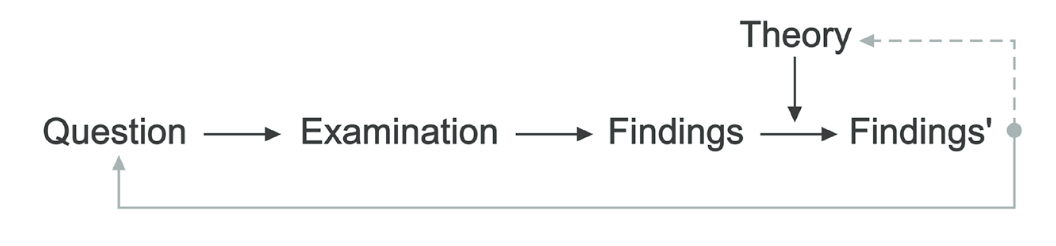
\includegraphics[width=10cm]{pictures/Theory/analytical_theory.png}
    \caption{The "Theory as analytical tool model".}
    \autocite[p. 133]{beck_examining_2016}
\end{figure}

\section{Objectifying meaningfulness}
The way we position ourselves to understand meaningfulness in museums, is by comparing the three place-centred approaches accounted for in Chapter 3; Hybrid place, place as a dialogue and Sense-making. To design a meaningful experience, we are interested in three things:

\begin{itemize}
    \item How do the installation fit into the museum agenda and exhibition space?
    \item In what degree is the interactive elements in the installation dialogic? (e.g. how well do the elements stimulate or trigger conversations, reflections.)
    \item and, How well does the installation disseminate the message conveyed?
\end{itemize}

This is how \emph{the framework without a name} proposes how one can design meaningful interactive experiences in a museum space. The first iteration on what this would look like is evident in Figure 4.2, where the three theoretical approaches together fulfill three ways to capture behaviour and interactions between visitor and interactive installation, as an attempt to objectify meaningfulness as a quality you can design for. 

\begin{figure}[H]
\centering
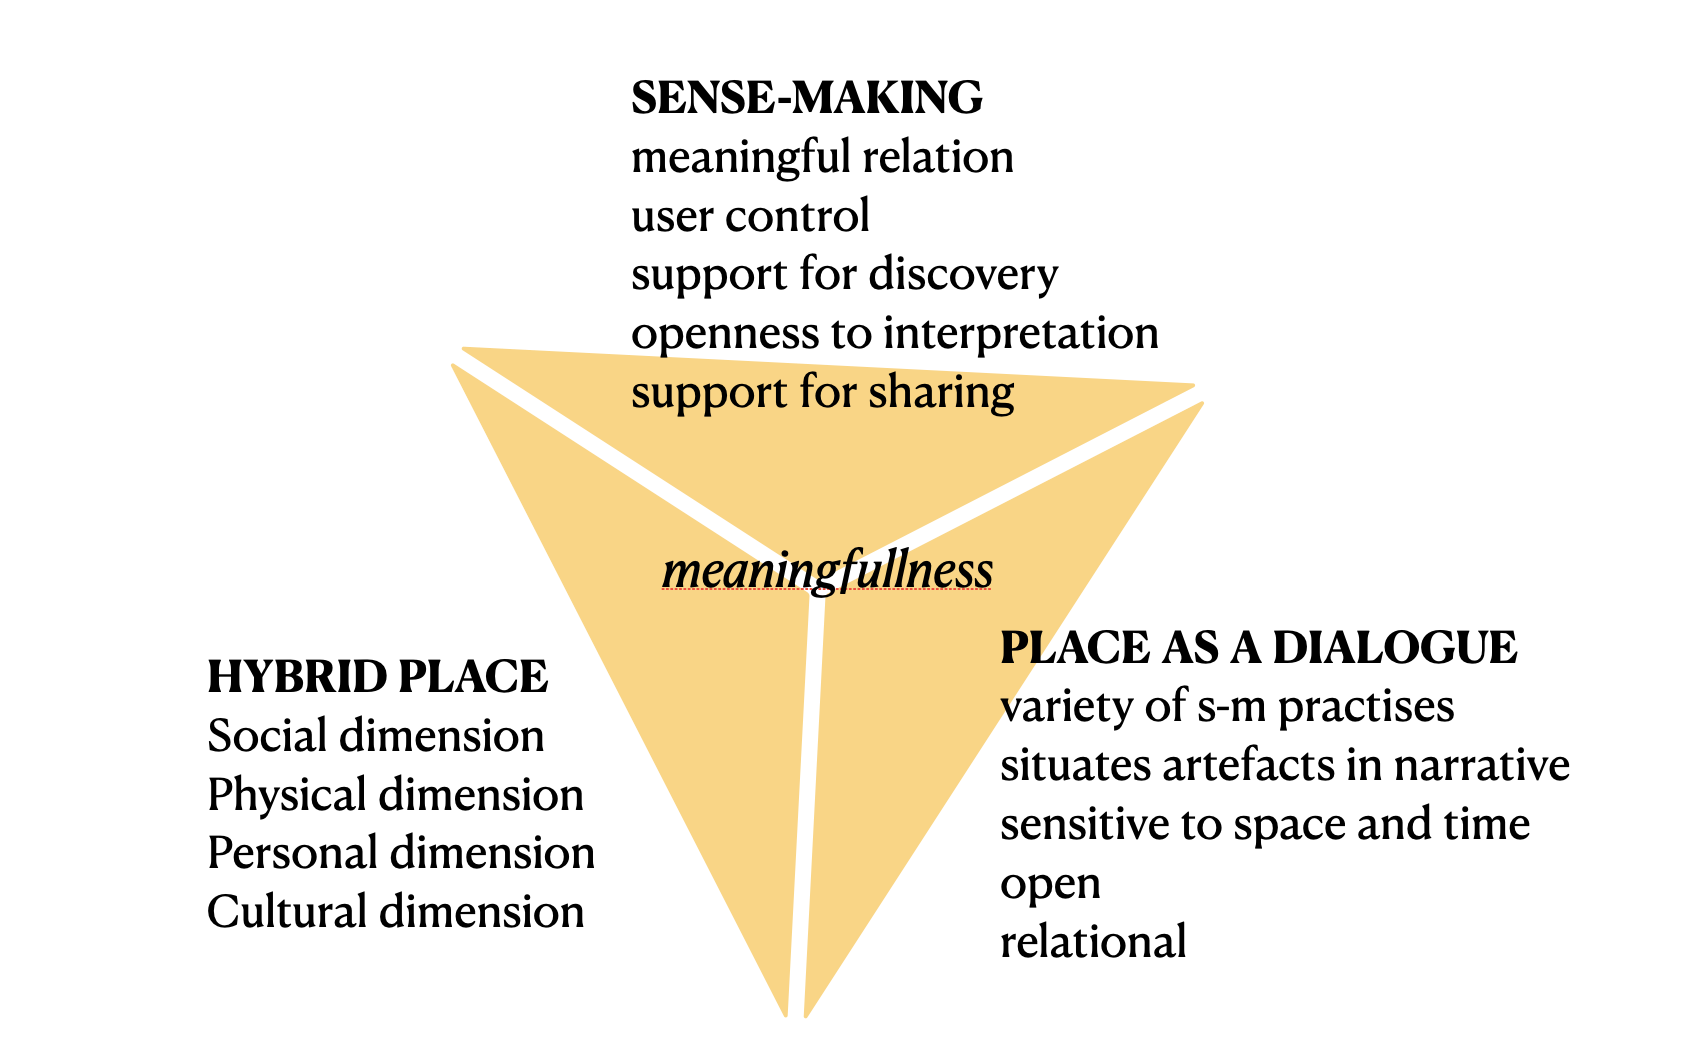
\includegraphics[width=12.5cm]{pictures/Theory/triangle_first.png}
\caption{Early representation of the framework}
\end{figure}

As we can see in Figure 4.2, I borrow four dimensions from the Hybrid Place approach; the \emph{physical, social, personal and cultural}, as a way to portray/ map out the installation in relation to its environment. Addressing the first bullet-point; how do the installation fit into the museum agenda and exhibition space? From the Place as a Dialogue approach I borrow five principles; the \emph{in the centre of a variety of sense-making practises, situates artefact in narrative, sensitive to the peculiarities of space and time, open, and relational}. This way we can look at the relationship between the visitor and exhibition, addressing the second bullet-point; In what degree is the interactive elements in the installation dialogic? (e.g. how well do the elements stimulate or trigger conversations or reflections). And lastly from the Sense-making approach I borrow five strategies; \emph{meaningful relation to target, user control, support for discovery, openness to interpretation and support for sharing}. This way we can look closer at the relationship between the installation, the exhibition and the visitor, addressing the third bullet-point: how well does the installation disseminate the message conveyed. As expressed in Figure 4.3, you will see how the theoretical approaches (Hybrid, Place, or Sense) respectively aim to provide and complement a layered understanding - objectifying meaningfulness as a quality you can design for in museum spaces.

\begin{figure}[H]
\centering
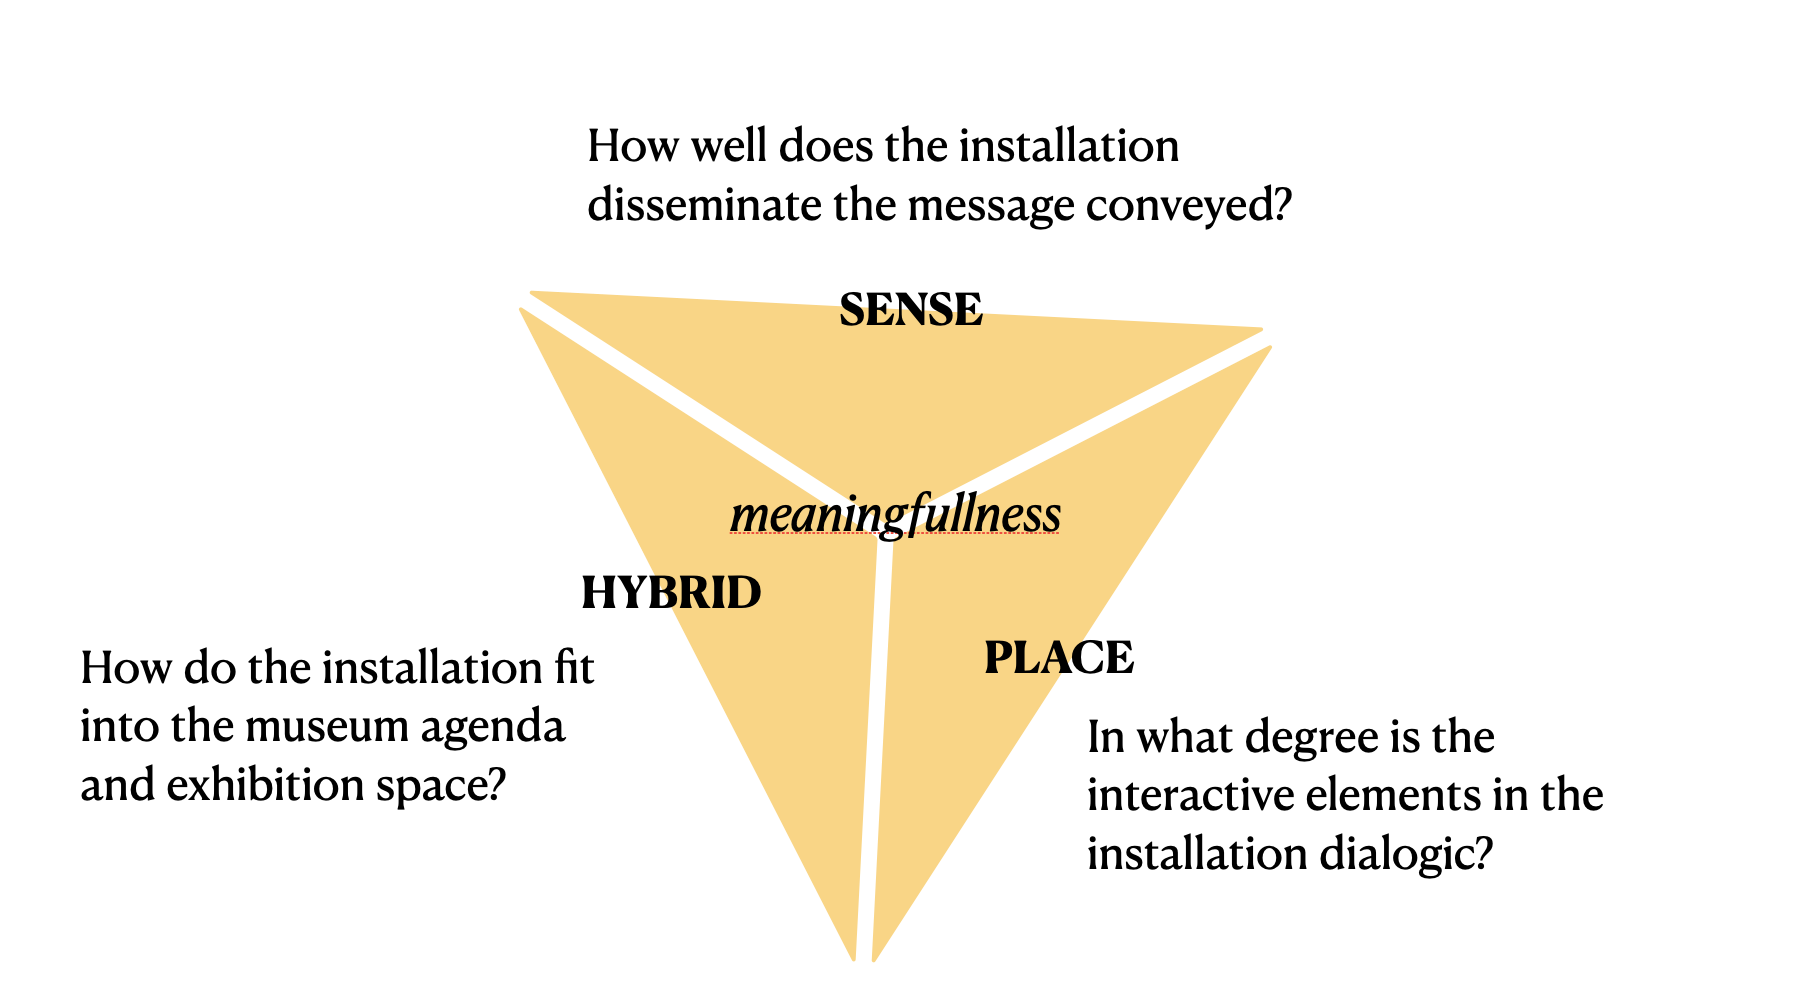
\includegraphics[width=12.5cm]{pictures/Theory/triangle_explicit.png}
\caption{Early declarative representation of framework}
\end{figure}

There is yet much potential and refining to be uncovered after applying the framework in practise. The main challenge and concern is to see how the three approaches can compare and be put together. After visiting and examining interactive installations, we will first have to categorize the installations to see which dimensions, principles and strategies that aligns with it. Then we will have the means to look at the overall trends for the respective approach, before we embark to trying to identify the meaningful relations between the approaches. In dialogue with my supervisor, early thoughts on how to compare and deduce the interplay between the three approaches was to make radar charts and heat-mapping based on the inherent data. These are all concerns that will need to be addressed in an analytical phase of the thesis project, and is accounted for in Chapter 7. 

\begin{figure}[H]
\centering 
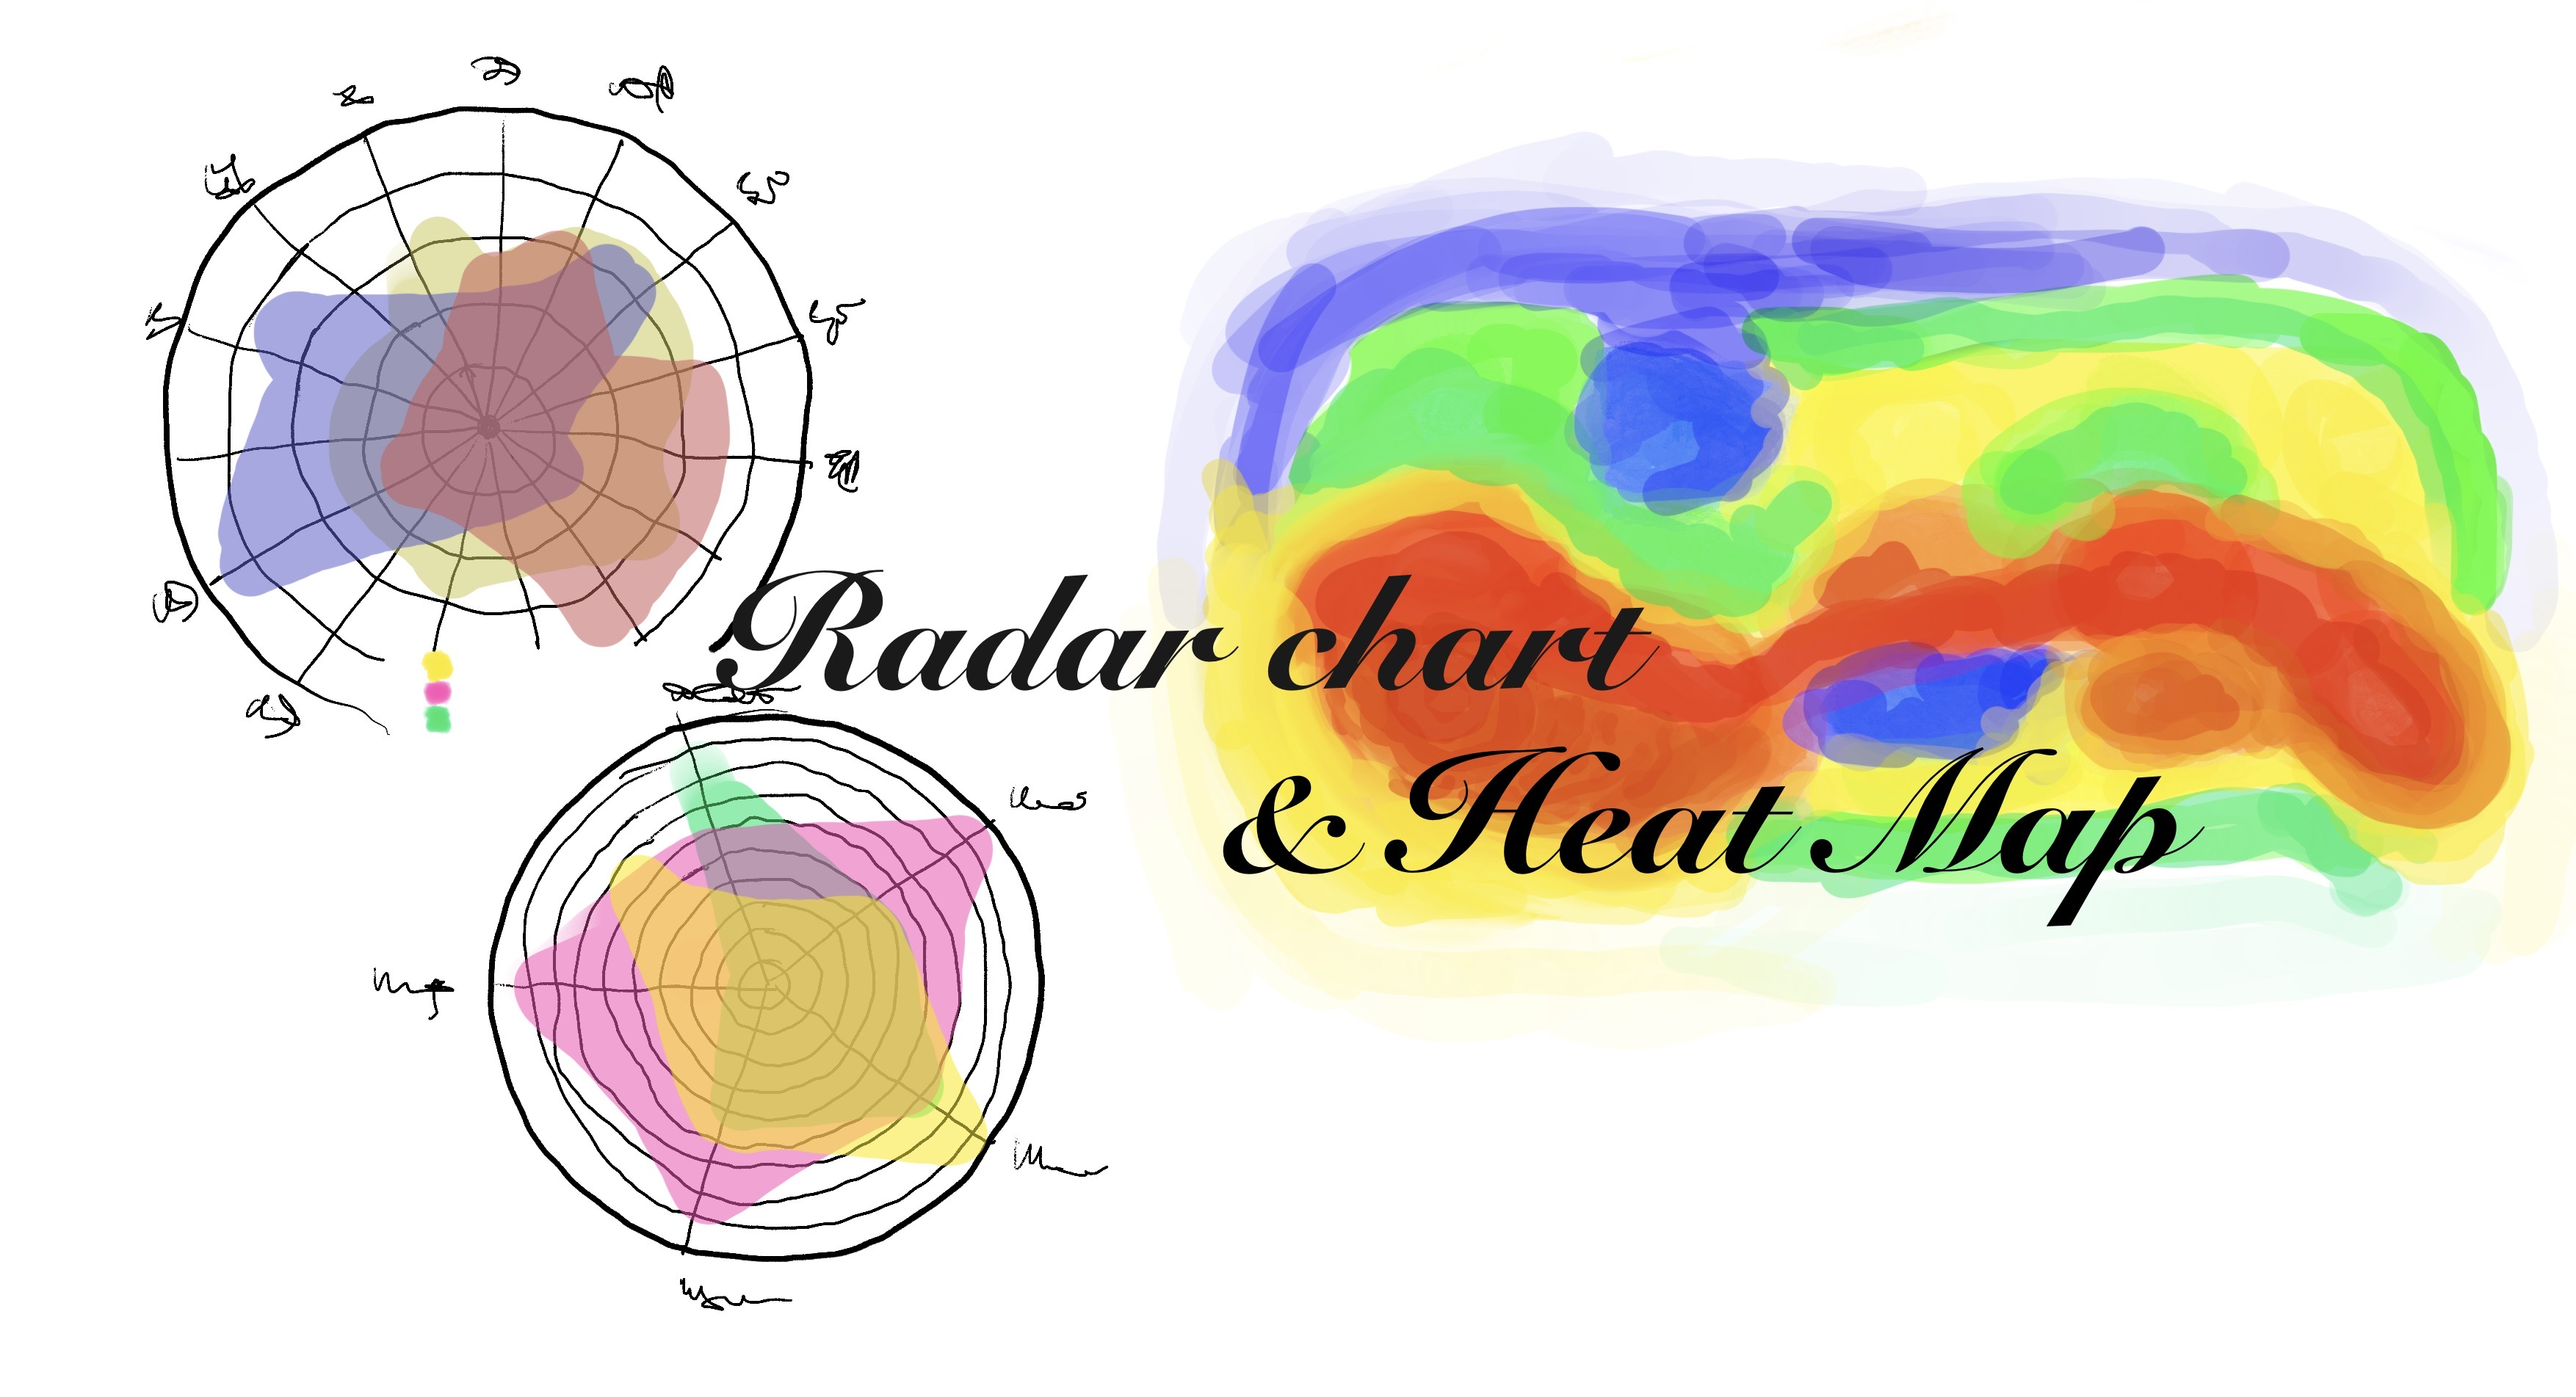
\includegraphics[width=10cm]{pictures/Theory/radar_and_heatmap.jpeg}
\caption{Early thoughts on framework interplay}
\end{figure}

\section{Patterns revealing meaningful relations}
Inspired by the works of \autocite{pattern_language_1977}, on pattern languages, and the more philosophical timeless way of building \autocite{Alexander_book}, I have worked to see how the framework could produce practical, hands-on knowledge on interactions in the museum space. Patterns representing, or documenting, dialogic interactions between the visitor and interactive exhibition artefacts have been an early appeal and seemed like a fitting research contribution to the overarching research question of how one can design for meaningfulness in a museum space addressing sustainability.

In a paper examining the experiences and expectations that HCI researchers who have been involved in Pattern Language research, \autocite{pan_pattern_2013} provide some overall reflections and several possible directions on the use of pattern language in HCI. Pattern language was first introduced by Christopher Alexander and his colleagues in their book \emph{A pattern language} with regards to timeless architecture and urban design \autocite{pattern_language_1977}. A pattern language is a group of patterns that attempt to give a solution to a recurring problem, and although there was no detailed exploration of how to apply pattern language to the filed of HCI, Norman claimed that Alexander’s work had particularly influenced him \autocite[p. 1990]{pan_pattern_2013}. Later on, Thomas Erickson suggested using Pattern Language as a meta-language to support interdisciplinary work in HCI and interaction design. He describes three main advantages of pattern language in interaction design, namely concreteness and bounding to the situation, reusable in different domains, and amendable to generalization across workplace \autocite[p. 1991]{pan_pattern_2013}. Since then, the notion of pattern language as a \emph{lingua franca} has been repeated and advocated by HCI researchers and practitioners in supporting interdisciplinary work. The application of pattern language in interaction design has been further investigated and examined by other HCI researchers and practitioners, such as \autocite{zimmerman_designing_2009}'s article \textit{Designing for the self: Making products that help people become the person they desire to be}. Zimmerman's research has mainly focused on the use of pattern language to document conventions and analyze user behaviors in user research \autocite[p. 1991]{pan_pattern_2013}. As Zimmerman's discuss his use of design patterns, they ended up to deviate fairly widely from the intended purpose of documenting and making explicit design conventions, while instead worked to illuminate the link between the application of product design theory and the designed artefact, allowing the similarities in the application of theory across the very different design projects to be seen \autocite[p. 402]{zimmerman_designing_2009}.

% Need a little explanation on the Figure heeeere <3 

\begin{figure}[H]
\centering 
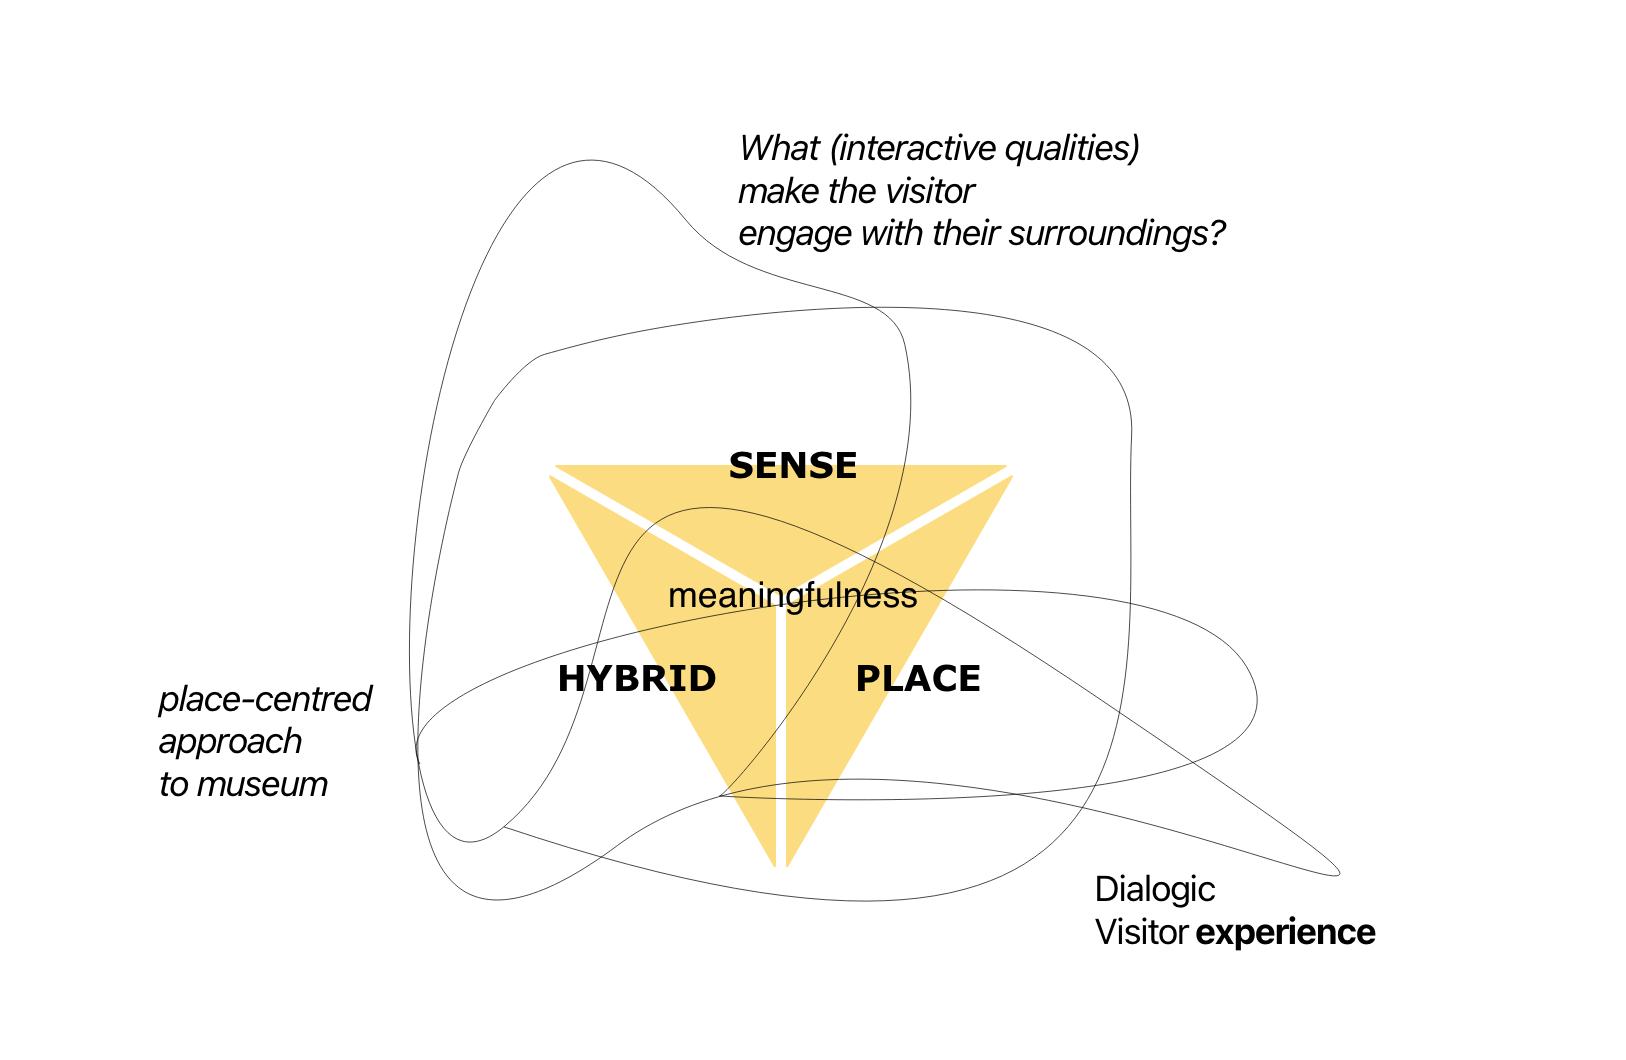
\includegraphics[width=13cm]{pictures/Theory/early_iteration_framework.png}
\caption{Early iteration on identifying meaningful relations}
\end{figure}


Truly inspired and following the work of Christopher Alexander, I will present the philosophical background of this thesis's framework based on Alexander's writings in his book The Timeless Way of Building. First, knowing, from the book's chapter 4, that any town or building gets its character from those events and patterns of events which keep happening there the most; and that the patterns of events are linked, somehow, to space \autocite[p. 81]{Alexander_book}. Then, in chapter 5: \textit{patterns of space}, we are presented with what aspects of the space it is that correlate with the events before introducing the "structure", or "logic" of making a pattern. In the next paragraphs, I will go through Alexander's reasoning for understanding the structure of relationships existing, and rooted in, space, relating it to the museum context that we are interested in the scope of this thesis.

Alexander write: \emph{"On the geometric level, we see certain physical elements repeating endlessly, combined in an almost endless variety of combinations. And each of these elements has a specific pattern of events associated with it. But this picture of space does not explain how - or why - these elements associate themselves with definite and quite specific patterns of events. Let us therefore look more carefully at the structure of the space from which a building or a town is made, to find out what it really is that is repeating there. Beyond its elements each building is defined by certain patterns of relationships among the elements. Evidently, then, a large part of the "structure" of a building or a town consist of patterns of relationships."} \autocite[p. 82-83]{Alexander_book}.

Based on readings and initial fieldwork expedition to the museum space of Klimahuset, we can already start "seeing" repeating elements and specific patterns of events associated with it, distinctively found in all museums linked to exhibition practise. The most obvious one is the artwork, where related patterns of events would be something like; looking at the artwork, reading the sign plaque, moving closer to study a detail, or thinking or reflecting alone or with a group. As visualized in Figure 4.7, we can count six arrows, each representing a related pattern of event to the artwork - which just come to show that there is more happening than meet the eye at first glance. These six patterns of events are, of course, only surface-level and purely based on early-stage domain knowledge. However, as a designer working with museum experience design, these are the types of interactions you would want to support or work to extend, add to, or strengthen the relation. To design a meaningful experience, in comparison to designing an engaging experience, should not necessarily be about designing the most innovative installation ever - it should instead aim to extend, support, add or strengthen the already existing patterns of events - therefore securing a more tightly coupled link to the artefact's or exhibition's discourse and agency.

\begin{figure}[H]
\centering 
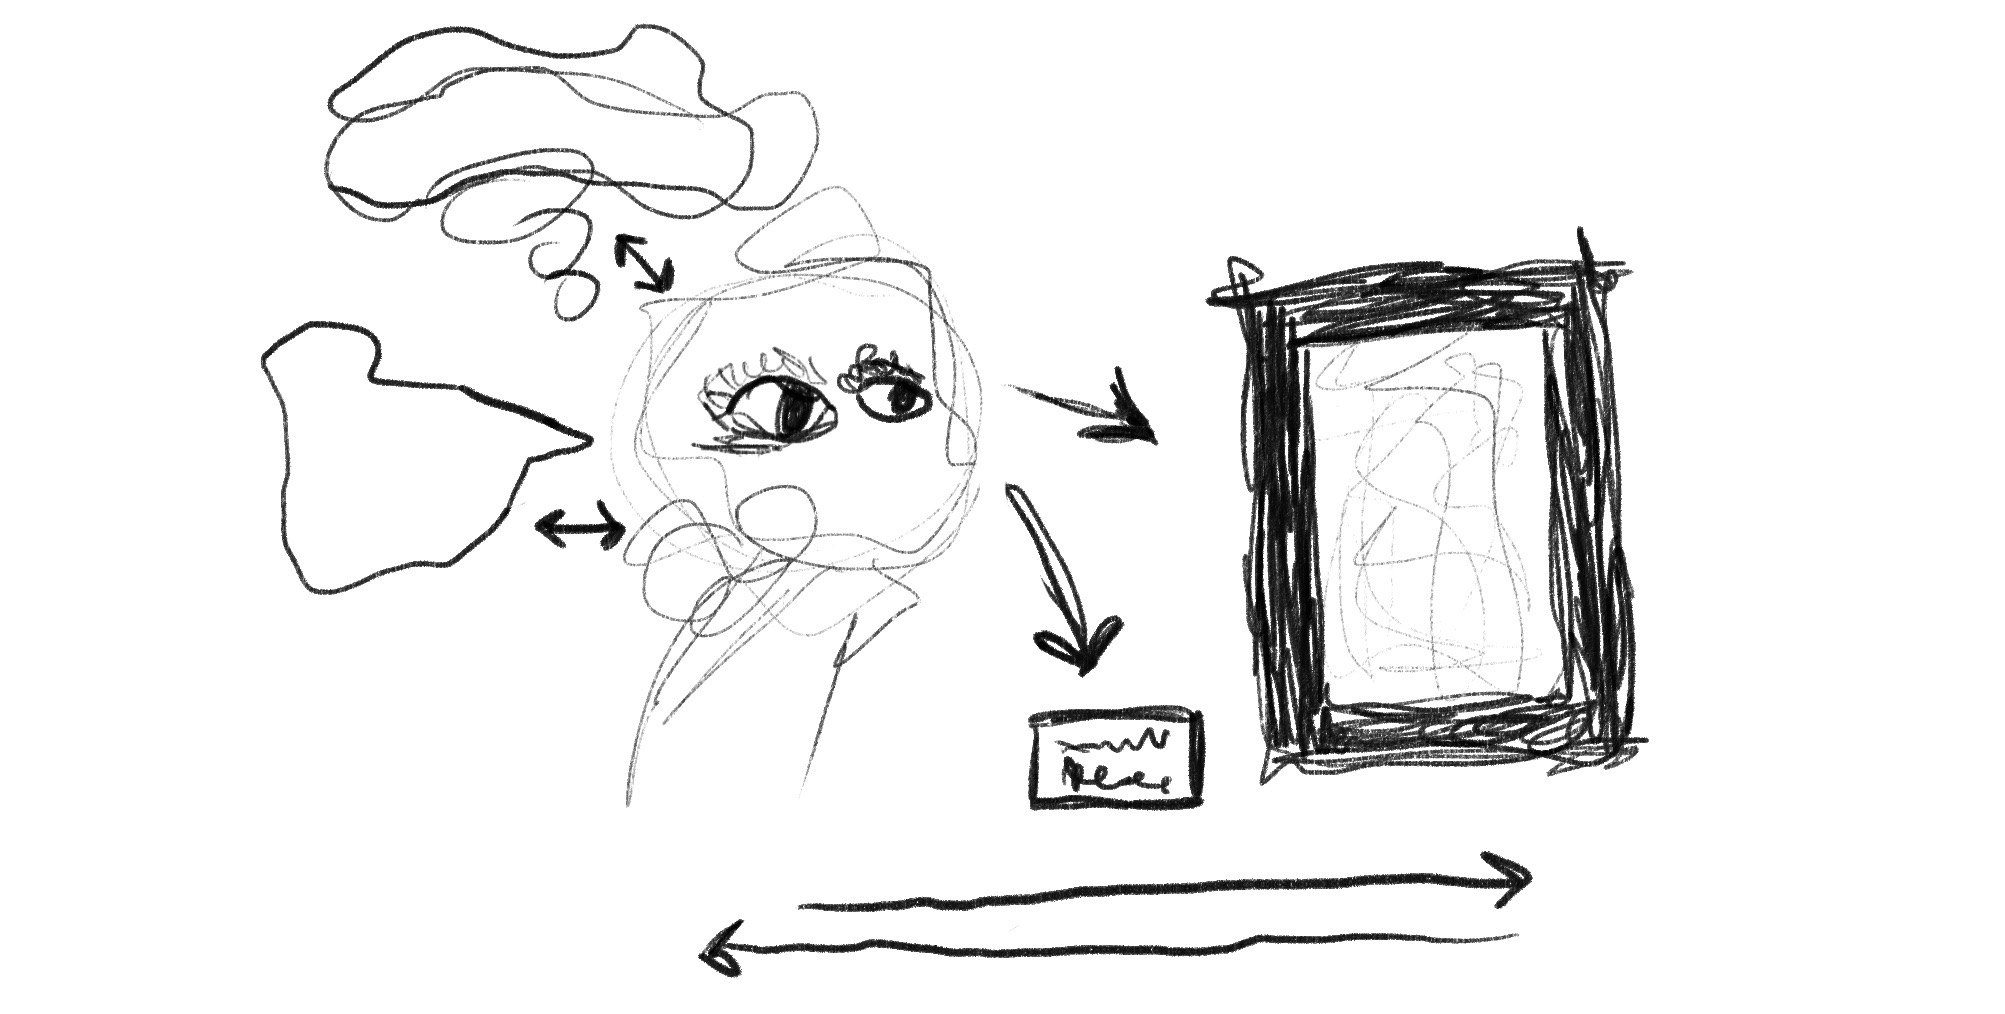
\includegraphics[width=10cm]{pictures/Theory/artwork_pattern.jpeg}
\caption{Surface-level patterns of events related to an artwork}
\end{figure}

Alexander continues: \emph{"At first sight it seems as though these patterns of relationships are separate from the elements. When we look closer, we realize that these relationships are not extra, but necessary to the elements, indeed a part of them. When we look closer still, we realize that even this view is still not very accurate. For it is not merely true that the relationships are attached to the elements: the fact is that the elements themselves are patterns of relationships. And finally, the things which seem like elements dissolve, and leave a fabric of relationships behind, which is the stuff that actually repeats itself, and gives the structure to a building or a town."} \autocite[p. 85-89]{Alexander_book}.

Again, based on readings and initial fieldwork efforts in the process of getting to know the museum domain, I believe there lies value and opportunities for designers and practical researchers in abstracting the exhibition artefacts from what they are - to decompose them to see what they represent, and what they do. That way, we can see the user behavior already existing in the museum space. This could be useful in conceptual stages in the design process when deciding where, how, and why the new designed artefact fits \emph{into} the exhibition. It also opens up a new design space for seeing and understanding the existing exhibition experience, so when the question of the thematic agency or discourse the new designed artefact should represent - the designer have the opportunity to comment on or support the current exhibition. This way, \emph{the framework without a name} serve both an identifying and analytical function in terms of the intended knowledge production in use.

Then, comes Alexander's working explanation for how one can create a pattern: \emph{"Each one of these patterns is a morphological law, which establishes a set of relationships in space. This morphological law can always be expressed in the same general form:}

\begin{quote}
\centering $X \rightarrow r (A, B, ...)$,
\end{quote}

\emph{
which means: Within a context of type X, the Parts A, B, ... are related by the relationship r. "}\autocite[p. 90]{Alexander_book}.

As will become evident in Chapter 7: Analysis, we will see how one can leverage the data-set so that we can start the process of making patterns from the interactive installations the research buddies and I have visited.

\emph{"Of course the patterns vary from place to place, from culture to culture, from age to age; they are all man-made, they all depend on culture. But still, in every age and every place the structure of our world is given to it, essentially, by some collection of patterns which keeps on repeating over and over and over again. These patterns are not concrete elements, like bricks and doors - they are much deeper and more fluid - and yet they are the solid substance, underneath the surface, out of which a town or a building is made."} \autocite[p. 100]{Alexander_book}.

And just like that, museums speak different fictions and addresses different discourses. The power of identifying patterns and opening up a new design space simply provides a better foundation to create exhibition design for the specific museum context you're working with. By seeing and working from the structural, place-centred logics in the space, the designer would have the possibility to position the new exhibition design to cultivate the museum culture and agency. Thus, meaningful not only in the artefact, but also, the experience. These are the notions on the knowledge production the \emph{framework without a name} is designed and intended to produce. There is yet much potential and refining to be uncovered after applying the framework in practise. In the next Part of this thesis, the Design Process, we will account for following the methodological RtD approach, visiting several museums and different exhibitions and installations. \emph{The framework without a name} and its application will be showcased and refined in Chapter 7. 